\documentclass[11pt]{article}
\usepackage{deauthor,times,graphicx,subcaption}
%\graphicspath{{figs/}}


\begin{document}
\title{Operating systems support for data management \\ on modern hardware}
\author{Jana Giceva \\ Imperial College London \\ j.giceva@imperial.ac.uk}
\maketitle

\begin{abstract}
For decades, database management systems have found the generic interface, policies and mechanisms offered by 
conventional operating systems at odds with the need for efficient utilization of hardware resources. The 
existing approach from the OS-side of "one-size-fits-all" interface and policies fails to meet modern data 
management workload's performance expectations, and the "overwriting the OS policies" approach from the 
DB-side does not scale with the increasing complexity of modern hardware and deployment trends.
 
In this article, we present two approaches on how to improve the systems support for database engines. First, 
we extend the OS with a policy engine and a declarative interface to improve the knowledge transfer between 
the two systems. Such extensions allow for easier deployment on different machines, more robust execution 
in noisy environments and better resource allocation without sacrificing performance guarantees. Second, 
we show how we leverage a novel OS architecture to develop customized OS kernels that meet the needs of 
data management workloads. Finally, we discuss how both approaches can help to address the pressing 
challenges for data processing on heterogeneous hardware platforms.
\end{abstract}

%\section{Introduction}  
\label{s:intro}
The past decade has observed a surge in the design and deployment of 
decentralized systems. A key reason for this surge is the growing desire in 
the society to have self-governing democratic financial systems that are not 
under the control of a privileged set of entities. A central control often 
translates to a forced trust model with limited provision to support 
transparency and accountability. The adoption of Blockchain, for example, 
is a by-product of the ability to break away from the forced-central control 
in a trust-worthy fashion~\cite{blockchain-book}. The emerging blockchain 
platforms facilitate a reliable execution of any digital contracts 
(i.e., transactions) in a decentralized manner despite the existence of malicious 
actors. At the core of any blockchain platform is a Byzantine 
fault-tolerant (\BFT{}) consensus protocol and a tamper-proof replicated 
ledger~\cite{bedrock,blockchain-book,scalable-ledger}. The \BFT{} 
protocol helps to achieve {\em consensus} on the order of incoming client 
requests among all the replicas, while the ledger logs this agreement. 

Traditional \BFT{} protocols expect a {\em permissioned} system where the 
identities of all the replicas (i.e., participants) are known prior to any 
consensus as they rely on having a verifiable voting right in a democratic 
setting. These protocols rely on a {\em communication-oriented} consensus 
model, where all the participants exchange endorsements across multiple 
rounds before they can reach a decision~\cite{sharper,pbftj,ahl,poe,rcc,geobft,flexitrust,ringbft,mirbft,basil,hotstuff}.
In these protocols, a system of $\n{}$ replicas can reach a common decision 
if at most $\f{}$ of them are malicious, such that $\n{} \ge 3\f{}+1$. 
The $\n{}$ parties are said to reach a decision when at least a majority 
of honest parties agrees to that decision. This decision is logged by 
requiring all the agreeing parties to {\em sign} the decision. Hence, the 
reached decision is considered {\em tamper-proof} because it has support 
of a majority of honest participants.

Despite being around for more than two decades, traditional \BFT{} protocols 
did not see any major practical applications until the introduction of 
blockchain technology. We attribute {\em two} key factors for this lack of 
adoption. (i) To ensure that the malicious participants do not spawn multiple 
identities, these \BFT{} protocols need an authority (i.e., {\em a forced 
trust gateway}) to verify and register every participant to verify every 
vote~\cite{sybil-attack}; some participants may find this intrusive if they 
do not want to reveal their personal information. (ii) To overwrite the ledger, 
malicious participants just require access to the private keys of honest 
participants. In a sense, the proof of the validity of the ledger is not 
self-contained, and it operates on the assumption that the private-keys 
are kept safe externally indefinitely.

To resolve these challenges, initial blockchain platforms such as 
Bitcoin~\cite{bitcoin} and Ethereum~\cite{ether} offer a {\em permissionless} 
model of consensus. These systems employ the {\em Proof-of-Work} (\PoW{}) 
protocol~\cite{bitcoin,ether}, which follows a {\em computation-oriented} 
consensus model and requires all the participants to compete with each other 
and try to solve a complex puzzle. Whichever participant solves the puzzle 
first gets to add a new entry ({\em block}) to the ledger. As a result, 
\PoW{} protocol eliminates the three challenges seen by traditional \BFT{} 
protocols. (i) Malicious participants can spawn multiple identities, but what 
actually matters is the available compute power. (ii) Each block includes 
the hash of the previous block; overwriting the ledger requires recomputing 
all the blocks making it computationally infeasible. (iii) Since reaching the 
consensus is based on presenting the proof of work that is embedded on the 
ledger (i.e., self-contained), there is no longer any need for external 
safe-keeping of private keys to sign endorsements.

These properties offered by \PoW{} protocol help blockchain platforms to 
design a {\em decentralized economy}, where any person can participate in the 
consensus process, and the economy has a self-generating currency to monetize 
its participants. Monetizing the participants is necessary as the \PoW{} 
protocol expects the participants to spend their resources to solve a complex 
puzzle. Clients of the Bitcoin platform, create transactions that exchange 
Bitcoins and send them to the participants (miners) in the \PoW{} protocol. 
These miners check if the transaction is valid; the client has sufficient 
Bitcoins to transfer. If the transaction is valid, they run \PoW{} protocol to include 
this transaction in the ledger. The winning miner of \PoW{} gets a portion of 
the client's Bitcoin as {\em fees}, while the mining process (\PoW{}) mints  
new tokens to fund the economy. This new token is transferred to the winning 
miner's account and is recorded as a transaction in the block.

The key challenge with platforms like Bitcoin is their {\em practicality}. 
These platforms have abysmally low throughput in the order of $10$ transactions 
per second in part due to inadequate choice of small block sizes. Furthermore, as 
more miners join the network, the complexity of the puzzle has to be increased. 
For example, the complexity of the current Bitcoin puzzle is so high that the 
miners work in large groups to have any positive probability of creating the 
next winning block~\cite{blockchain-book}. Moreover, as miners are competing 
with each other, it leads to massive wastage of computational resources (energy) 
as only the winning miner's efforts are recorded and rewarded. This results in an unsustainable ecosystem~\cite{badcoin,badbadcoin}.

We observe these challenges in the designs of existing \BFT{} protocols and 
blockchain platforms and envision a \DualChain{} system that learns from these 
models and eliminates their key challenges. Essentially, we aim to establish a 
new research agenda; a new field of hybrid consensus protocols that depart from 
competitive consensus to a collaborative consensus that is both resilient and 
sustainable. Our \DualChain{} architecture takes a step in this direction by 
running two consensuses on each client transaction while ensuring there is no 
increase in the latency observed by the client. Each client request is first 
ordered through a state-of-the-art \BFT{} consensus protocol ({\em commitment}), 
subsequently, this ordered request is engraved into the ledger through the 
\PoW-style consensus ({\em settlement}). Specifically, \DualChain{} causes no 
increase in commitment latency while improving the settlement latency observed 
by existing protocols. Ordering the client transaction through a \BFT{} consensus 
protocol first allows our \DualChain{} system to guarantee the following benefits: 
(i) clients receive low-latency responses, and (ii) \PoW{} participants no longer 
need to compete, resulting in a high-throughput sustainable chain. As a result, 
instead of employing the \PoW{} for consensus, we design a novel protocol that 
allows miners to collaborate. We refer to this paradigm as 
{\em Power-of-Collaboration} (\PoC{}). 

Our \PoC{} protocol splits the complex puzzle into disjoint slices and requires 
each miner to work on a distinct slice. This slice distribution significantly 
reduces the resource wastage and provides each honest miner with a reward 
for each new transaction added to the ledger. As each ledger entry is added 
collaboratively, any malicious entity that wishes to overwrite the ledger 
needs to match the computational power of all the existing miners making it 
practically impossible. These features of our \DualChain{} system make it 
lucrative; its design is the bedrock for a secure and efficient decentralized 
economy.


\section{Introduction}

Generally, today's operating systems multiplex applications with little to no information 
about their requirements. They migrate, preempt, and interrupt threads on various cores,
trying to optimize some system-wide objectives (e.g., load balancing the work queues
on individual cores and across the NUMA nodes~\cite{Lozi:eurosys16}). As such, the OS
has no notion about how its decisions affect the performance of the applications 
primarily due to the limited communication between the two layers~\cite{cod:2013}. 

As a result, database engines that run on commodity operating systems often experience
performance problems, which are caused by the generic OS policies~\cite{Stonebraker:1981}. 
First, when executing in a noisy environment alongside other applications, the 
default OS policies for resource management can often cause performance 
degradation~\cite{Shoal} or inefficiencies in resource usage~\cite{Giceva:damon16,Lozi:eurosys16}. 
Second, even when running in isolation, databases often override the generic OS policies
(e.g., by pinning threads to cores, allocating memory from a particular NUMA node, or 
pinning pages to avoid swapping, etc.~\cite{Porobic:icde14,Kimura:2015}). The 
problem with such user-side optimizations is that they are often tailored to a 
specific architecture, which makes portability to other platforms a daunting
task~\cite{Makreshanski:vldb15,satish:sigmod10}. 
Third, frequently the applied optimizations are fragile as they rely on assumptions on
what the OS kernel mechanisms and policies do (e.g., HyPer~\cite{HyPer} leverages
an efficient OS-assisted snapshotting). Consequently, any change in the OS policies
can cause performance bugs that are difficult to identify and debug.

In light of modern hardware trends of increased hardware heterogeneity and machine 
diversity, pushing all the complexity up to the developer or within the database 
engine does not scale. Furthermore, as databases are often deployed in the cloud,
alongside other applications and tasks, they can no longer assume to have full
ownership of the underlying machine's resources and any scheduling decision they do
may be at odds with the noisy system environment and result in unpredictable 
performance.

In this article we argue that it is time to revisit the interface between operating
systems and databases and address the modern challenges in a holistic manner crossing
various layers across the systems stack. More specifically, we propose a solution that
first addresses the semantic gap that exists between the database engine and the 
operating system by leveraging (1) a powerful declarative interface between the two
layers allowing for bi-directional information flow, and (2) an OS policy engine that 
unifies the knowledge present in the database (workload characteristics, access patterns,
cost models, data distribution, etc.) with the knowledge of the OS about the 
underlying hardware and the runtime system-state. 
Furthermore, we present a novel OS architecture that allows for OS kernel customization
(i.e., policies, mechanisms and services) based on the specific requirements of 
the database system or its workloads. Our design is inspired by recent advancements
in operating systems, which enable systems to run a specialized kernel on a subset
of the resources on a given machine. This enables the database to get considerably
more control over the full OS stack, which can then be tuned to achieve both better
performance and stronger guarantees. 
Finally, we argue how both design principles are suitable to target modern hardware 
resource dis-aggregation challenges, raising a few interesting research directions.

%\newcommand{\parai}[1]{\noindent\textit{#1}}

\section{Background}
\label{sec:background}

In this section, we recall the \SecAgg protocol first, then the compression methods that we wish to adapt to \SecAgg, namely, scalar quantization, pruning, and product quantization.

\subsection{Secure Aggregation}
\label{subsec:secagg}

\SecAgg refers to a class of protocols that allow the server to aggregate client updates without accessing them individually. While \SecAgg alone does not entirely prevent client data leakage, it is a powerful and widely-used component of current at-scale cross-device FL implementations~\citep{kairouz2019advances}. Two main approaches exist in practice: software-based protocols relying on Multiparty Computation (MPC)~\citep{bonavitz2019federated,bell2020secure,LightSecAgg}, and those that leverage hardware implementations of Trusted Execution Environments (TEEs)~\citep{huba2021papaya}. 
% While these approaches have substantial differences, they impose similar constraints on compatible update compression techniques: operating over finite fields and assuming that aggregation commutes with decompression.


\SecAgg relies on additive masking, where clients protect their model updates $g_i$ by adding a uniform random mask $m_i$ to it, guaranteeing that each client’s masked update is statistically indistinguishable from any other value. 
% Masks are generated so that when all the masked client updates are aggregated by the server (typically through addition), the server obtains the exact aggregate (e.g., the sum of updates). 
At aggregation time, the protocol ensures that all the masks are canceled out. For instance, in an MPC-based \SecAgg, the pairwise masks cancel out within the aggregation itself, since for every pair of users $i$ and $j$, after they agree on a matched pair of input perturbations, the masks $m_{i,j}$ and $m_{j,i}$ are constructed so that $m_{i,j}=-m_{j,i}$.
Similarly and as illustrated in Fig.~\ref{fig:secagg_summary}, in a TEE-based \SecAgg, the server receives $h_i = g_i + m_i$ from each client as well as the sum of the masks $\sum_i m_i$ from the TEE and recovers the sum of the updates as
% by unmasking the aggregated updates as 
%\begin{equation*}
$
      \sum_i g_i = \sum_i h_i - \sum_i m_i.
$
%\end{equation*}
We defer the discussion of DP noise addition by \SecAgg protocols to Section~\ref{sec:discussion}.

\para{Finite Group.}
\SecAgg requires that the plaintexts---client model updates---be elements of a finite group, while the inputs are real-valued vectors represented with floating-point types. 
This requirement is usually addressed by converting client updates to fixed-point integers and operating in a finite domain (modulo~$2^p$) where $p$ is typically set in prior literature to 32 bits. The choice of \SecAgg bit-width~$p$ must balance communication costs with the accuracy loss due to rounding and overflows.

% The other constraint is due to the fact that SecAgg is designed so that the server sees only the aggregate (the sum or the weighted sum) of individual gradients, plus some noise injected by a differentially private mechanism. A drop-in decompression operator $D$ must commute with SecAgg, or be close to being one:
% \[
% D\left(\sum_i g_i+\mathrm{noise}\right) \approx \sum_i D(g_i)+\mathrm{noise}. 
% \]
\para{Minimal Complexity.}
\looseness=-1
TEE-based protocols offer greater flexibility in how individual client updates can be processed; however, the code executed inside TEE is part of the trusted computing base (TCB) for all clients. In particular, it means that this code must be stable, auditable, defects- and side-channel-free, which severely limits its complexity. Hence, in practice, we prefer compression techniques that are either oblivious to \SecAgg's implementation or require minimal changes to the TCB.

% In the remainder of the paper, we focus on the TEE-based approach for its simplicity, scalability and compatibility with asynchronous FL. relies on random masking to encrypt the local model updates. The server then incrementally aggregates the encrypted updates and unmasks the aggregate using the sum of the random masks transmitted by the Trusted Secure Aggregator (TSA) that sits within the TEE. More formally, let us denote $??$ a local client update, represented in floating-point precision, generally \texttt{fp32}. First, the client converts $??$ to a fixed point representation. Then, the client generates a random mask $m \in \Z^d$ and computes the sum modulo a number. \ashkan{TODO}

% SecAgg protocols prevent the server from accessing individual client updates by aggregating them and transmitting only the aggregate to the server. While such mechanisms alone do not entirely prevent data leakage, they constitute a vital component of cross-device FL implementations~\citep{kairouz2019advances}. SecAgg relies either on Secure Multiparty Computation \cite{bonavitz2019federated,so2021secure} or on a Trusted Executed Environment or TEE~\citep{huba2021papaya}. In the remainder of the paper, we focus on the TEE-based approach for its simplicity, scalability and compatibility with asynchronous FL.

% TEE-based SecAgg relies on random masking to encrypt the local model updates. The server then incrementally aggregates the encrypted updates and unmasks the aggregate using the sum of the random masks transmitted by the Trusted Secure Aggregator (TSA) that sits within the TEE. More formally, let us denote $??$ a local client update, represented in floating-point precision, generally \texttt{fp32}. First, the client converts $??$ to a fixed point representation. Then, the client generates a random mask $m \in \Z^d$ and computes the sum modulo a number.

% Since the server, by design, never observes 

\subsection{Compression Methods}
\label{subsec:comp_methods}
In this subsection, we consider a matrix $W \in \mathbb{R}^{\cin\times \cout}$ representing the weights of a linear layer to discuss three major compression methods with distinct compression/accuracy tradeoffs and identify the challenges \SecAgg faces to be readily amenable to these popular quantization algorithms.

\subsubsection{Scalar Quantization}
\label{subsec:sq}

\looseness=-1 Uniform scalar quantization maps floating-point weight $w$ to $2^b$ evenly spaced bins, where $b$ is the number of bits. Given a floating-point scale $s > 0$ and an integer shift parameter $z$ called the zero-point, we map any floating-point parameter $w$ to its nearest bin indexed by $\{0,\dots, 2^b-1\}$:

\centerline{$w \mapsto \clamp(\round(w /s) + z, [0, 2^b - 1] ).$}

%
The tuple $(s, z)$ is often referred to as the quantization parameters (\texttt{qparams}).
With $b=8$, we recover the popular \texttt{int8} quantization scheme \citep{jacob2017quantization}, while setting $b = 1$ yields the extreme case of binarization \citep{courbariaux2015binaryconnect}. 
The quantization parameters $s$ and $z$ are usually calibrated after training a model with floating-point weights using the minimum and maximum values of each layer. 
% The accuracy drop due to this post-training quantization can be mitigated by pre-conditioning the network during training with techniques such as Quantization-Aware Training or QAT~\citep{krishnamoorthi2018quantizing}. 
% The quantization parameters can also be defined per-channel instead of per-layer to diminish the quantization error at the cost of a small memory overhead.
The compressed representation of weights $W$ consists of the \texttt{qparams} and the integer representation matrix $W_q$ where each entry is stored in~$b$~bits. 
Decompressing any integer entry $w_q$ of~$W_q$ back to floating point is performed by applying  the (linear) operator $w_q \mapsto s\times(w_q - z)$.

\para{Challenge.} 
The discrete domain of quantized values and the finite group required by \SecAgg are not natively compatible because of the overflows that may occur at aggregation time. For instance, consider the extreme case of binary quantization, where each value is replaced by a bit. 
We can represent these bits in \SecAgg with $p=1$, but the aggregation will inevitably result in overflows.

\subsubsection{Pruning}
\label{subsec:rp}

Pruning is a class of methods that remove parts of a model such as connections or neurons according to some pruning criterion, such as weight magnitude~(\cite{lecun1990optimal,hassabi1992second}; see \cite{Blalock20} for a survey). \cite{konen2016federated} demonstrate client update compression with random sparsity for federated learning. Motivated by previous work and the fact that random masks do not leak information about the data on client devices, we will leverage random pruning of client updates in the remainder of this paper. 
% as it is easiest to combine with SecAgg. 
% Let $\texttt{rand}$ be a function generating random entries in interval $[0, 1)$. 
% For a sparsity level $0\leq\rho\leq 1$, where $\rho=1$ yields a zero matrix, a client prunes entries~$w$ of~$W$ as: 
% % \karthik{TODO: decide on notation for rand}
% \[w \mapsto \begin{cases}
% 0 & \text{if } \texttt{rand()} < \rho \\ 
% w & \text{otherwise}.
% \end{cases}
% \]
% \sayan{should we number the equations ?}
A standard method to store a sparse matrix is the coordinate list (COO) format\footnote{See the  {torch.sparse documentation}, \url{https://pytorch.org/docs/stable/sparse.html}.}, where only the non-zero entries are stored (in floating point or lower precision), along with their integer coordinates in the matrix. 
This format is compact, but only for a large enough compression ratio, as we store additional values for each non-zero entry.
Decompression is performed by re-instantiating the uncompressed matrix with both sparse and non-sparse entries.

\para{Challenge.}
\modif{Pruning model updates on the client side is an effective compression approach} as investigated in previous work. However, the underlying assumption is that clients have different masks, either due to their seeds or dependency on client update parameters (\eg weight magnitudes). This is a challenge for \SecAgg as aggregation assumes a dense compressed tensor, which is not possible to construct when the coordinates of non-zero entries are not the same for all clients.

\subsubsection{Product Quantization}
\label{subsec:pq}


Product quantization (PQ) is a compression technique developed for nearest-neighbor search \citep{jegou2011product} that can be applied for model compression \citep{stock2019bit}. 
Here, we show how we can re-formulate PQ to represent model updates. 
We focus on linear layers and refer the reader to~\cite{stock2019bit} for adaptation to convolutions.
Let the \emph{block size} be $d$ (say, 8), the number of \emph{codewords} be $k$ (say, 256) and assume that the number of input channels, $\cin$, is a multiple of $d$. 
To compress $W$ with PQ, we evenly split its columns into subvectors or blocks of size $d \times 1$ and learn a \emph{codebook} via $k$-means to select the $k$ codewords used to represent the $\cin\times\cout/d$ blocks of $W$. PQ with block size $d=1$ amounts to non-uniform scalar quantization with $\log_2 k$ bits per weight.
% More formally, we first reshape $ W$ into a matrix of size $d \times \cin \cout / d$ and with a slight abuse of notation, we will also use  $W$ to denote the reshaped matrix and work only in the reshaped space. 
% Note that the reshaping approach applies to convolutional weights as well: e.g., for a 2D convolution with a kernel of size of $k_s$, we need to change the reshaping part to get matrix of size $d \times \cin\cout k_s^2/d$. 

The PQ-compressed matrix $W$ is represented with the tuple $(C, A)$, where $C$ is the codebook of size $k \times d$ and $A$ gives the assignments of size $\cin \times\cout / d$.
% \begin{align*}
% C & \text{    the codebook of size } k \times d,  \\ 
% A & \text{    the assignments of size }\cin \cdot\cout / d. 
% \end{align*}
Assignments are integers in $[0, k-1]$ and denote which codebook a subvector was assigned~to. 
To decompress the matrix (up to reshaping), we index the codebook with the assignments, written in PyTorch-like notation as
%\begin{equation*}
$
    \widehat {W} = C[A].
$
%\end{equation*}
% (appropriating a PyTorch-like notation) and perform a reshaping operation. PQ is naturally extensible to convolutional layers~\citep{stock2019bit}.

\para{Challenge.}
There are several obstacles to making PQ compatible with \SecAgg.  
First, each client may have a different codebook, and direct access to these codebooks is needed to decode each client's message.  
Even if all clients share a (public) codebook, the operation to take assignments to produce an (aggregated) update is not linear, and so cannot be directly wrapped inside \SecAgg. 
%In theory PQ is a linear operation, since we can encode each client's choice of codeword for a block with a 1-hot vector of length $k$, and com



\section{Background}

Databases and operating systems have a decades-long conflict when it comes to resource management and 
scheduling. Even though they initially started with the same goal -- providing efficient access 
of data written in files -- they took different approaches to addressing the problem. For many 
years this was not perceived as an issue as the two systems were targeting different 
workloads and machines. This shaped the role of monolithic databases and operating systems
as we know them today. 
However, the economic advantage of off-the-shelf hardware has led to today's situation where a 
database runs on top of conventional OS. The key problem is that the OS works with very little 
knowledge about the workload requirements and properties. Its primary role is to schedule 
resources among multiple applications and to provide isolation protection. As such, it sees the 
database as yet another program and offers the same generic mechanisms and policies, which often
lead to sub-optimal performance numbers.

Recent trends in both hardware architectures and resource dis-aggregation over fast network 
interconnects as well as economies of scale and deployment in the cloud are pressing both 
layers of the system stack to rethink their internal designs. The last decade, in particular, 
has seen profound changes in the available hardware as we reached the power wall limitation
and CPU frequencies stopped scaling. In response, hardware architects introduced multiple 
cores, heterogeneous compute resources and accelerators. Similarly, with the rise of the 
memory wall and the gap between DRAM and CPU frequencies, machines emerged with more 
complex cache hierarchies, non-uniform cache coherent memory, etc. Consequently, the 
system software (both DBs and OSs) has to adapt and embrace the new hardware landscape 
as an opportunity to rethink its architecture model and design principles.
For example, to improve performance, novel scheduling decisions within a database
engine~\cite{Leis:sigmod14,Porobic:icde14} and certain relational algorithms has 
shifted towards hardware awareness in modern machines~\cite{Polychroniou:2014,balkesen:15,wassenberg2011,muller:16}. 
Optimal use of resources today requires detailed knowledge of the underlying hardware 
(e.g., memory affinities, cache hierarchies, interconnect distances). 
Absorbing such complexity has now become the burden of the programmer and the 
problem gets further aggravated with the increasing diversity of micro-architectures. 

On the deployment side, in the age of cloud and server consolidation, databases can 
no longer assume to have a complete physical machine to themselves. They are 
increasingly more often deployed and offered as services on the cloud, where they
run alongside other applications. Consequently, the carefully constructed internal 
model of machine resources a database typically uses to plan the execution of its 
query plans and physical relational operators has become highly dependent on the 
runtime state of the whole machine. This state, however, is unknown to the database
and is only available in the operating system which has an overview of all 
active applications and orchestrates the resource allocation. 

In that context, we make the following observations. First, databases can no longer 
take full ownership of resource management, allocation and scheduling, partly because 
of increasing hardware complexity and portability issues, and partly because databases
today are running in noisy environments (e.g., in the cloud), alongside other applications.
Second, there is a big semantic gap between what each layer of the system stack knows --
the database engine about its workload properties and requirements and the operating 
systems about the underlying hardware and runtime system-state -- and the rigid 
interface between them does not allow for rich information flow. Fourth, the 
one-size-fit-all generic policies and mechanisms offered by the OS for a wide range 
of workloads do not work for performance sensitive applications, like data processing 
engines. And fifth, the heavy OS stack is no longer suitable for the new generation 
hardware, with heterogeneous (rack-scale) resource dis-aggregation. These are the 
issues we address as part of our work and discuss in the article.

%%!TEX root=../2022_IEEE_DEB_Vizier.tex

% %%%%%%%%%%%%%%%%%%%%%%%%%%%%%%%%%%%%%%%%
% \begin{figure}[t]
%   \centering
%   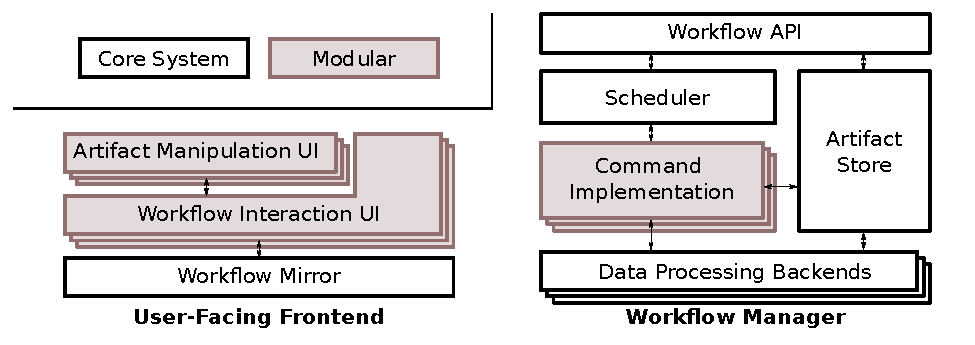
\includegraphics[width=0.7\textwidth]{graphics/systemarch}\\[-5mm]
%   \caption{Vizier's architecture, comprised of a user-facing frontend component and a backend component.}\label{fig:vizier-architecture}
% \end{figure}
% %%%%%%%%%%%%%%%%%%%%%%%%%%%%%%%%%%%%%%%%

%%%%%%%%%%%%%%%%%%%%%%%%%%%%%%%%%%%%%%%%%%%%%%%%%%%%%%%%%%%%%%%%%%%%%%%%%%%%%%%%
\pagebreak[4]
\subsection{Solution Overview}
\label{sec:solution-overview}

%%%%%%%%%%%%%%%%%%%%%%%%%%%%%%%%%%%%%%%%
\begin{wrapfigure}[12]{r}[0pt]{12cm}
  \centering
  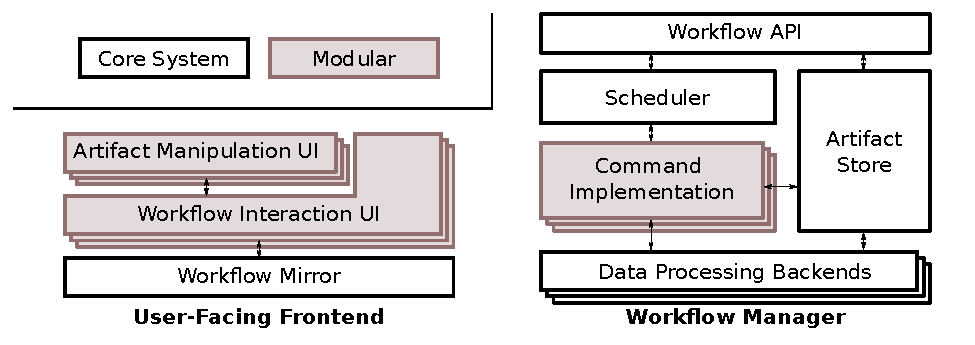
\includegraphics[width=0.7\textwidth]{graphics/systemarch}\\[-5mm]
  \caption{Vizier's architecture, comprised of a user-facing frontend component and a backend component.}\label{fig:vizier-architecture}
\end{wrapfigure}
%%%%%%%%%%%%%%%%%%%%%%%%%%%%%%%%%%%%%%%%
An overview of Vizier's architecture is shown in \Cref{fig:vizier-architecture}.
Addressing requirement \textbf{W1}, the central abstraction in Vizier is a workflow: a linear sequence of steps. % taken by the user in pursuit of a specific objective.
Unlike classical workflow systems, Vizier does not require users to explicitly declare information flow between steps.
Rather Vizier borrows the model employed in popular computational notebooks like Jupyter, where inter-cell communication occurs through a global state (artifacts) passed sequentially through steps.
Following notebook conventions, we refer to these steps as \emph{cells}, and the global state as a \emph{scope}, a map from artifact name to the version of the artifact valid at this point in the workflow. Vizier stores artifacts in common formats through a versioned \textbf{Artifact Store} (\Cref{sec:data-artifacts}), addressing requirement \textbf{A2}.
In \Cref{sec:vizier-workflows}, we formalize Vizier's workflow model, and show how we satisfy requirement \textbf{W3} by instrumenting how each cell interacts with the scope, allowing us to determine what artifact versions are valid.

Vizier's workflow semantics, paired with the versioned artifact store and workflow versioning (\Cref{sec:vizier-history}) addresses requirement \textbf{W2}. % as notebooks have a natural concept of logical order (the order of cells in the notebook) that can be adjusted over time.
% Adding workflow versioning  is sufficient to fully address the requirement.
In contrast, classical notebooks like Jupyter or Zeppelin rely on the global state of an interpreter for inter-cell communication.
Reverting this state to an earlier revision is challenging~\cite{zelnicki:2017:nodebook}, limiting their ability to satisfy requirement \textbf{W3}.
Vizier instead relies on its versioning system, allowing its \textbf{Scheduler} to automatically detect and re-evaluate stale cells (\Cref{sec:vizier-scheduler}).
To address requirement \textbf{A3}, we designed a light-weight uncertain data model that is implemented in Vizier in the form of \textit{caveats}, annotations on data that indicate uncertain values and rows  (\Cref{sec:data-docum-error}).

Addressing requirement \textbf{A1} requires modularity in both Vizier's front- and back-end components.
First, the user's interactions with a workflow and artifacts, whether through a scripting language, graphical interaction, or any other modality, need to be captured for replay (simultaneously addressing requirement \textbf{A4}). In Vizier this is achieved by requiring that every update to an artifact made through a particular modality has to be reflected as an operation in the workflow, i.e., a data update is translated into a workflow update.
Vizier manages a collection of \textbf{Command Implementations} that implement the logic behind these artifact transformations (\Cref{sec:multimodality}).
To streamline the implementation of commands, Vizier's data formats and transformations are built over standard \textbf{Data Processing Backends} like Apache Spark.
% For example, Vizier supports fine-grained provenance over datasets by encoding them as Spark data frames.

The frontend is implemented over a \textbf{Workflow Mirror} that uses websockets to reflect a live view of the workflow the user is editing.
Vizier automatically derives a default \textbf{Artifact Manipulation User Interface} for its notebook interface from each command's parameter schemas. This interface suffices for many templated commands, but the frontend can be further extended to provide a more customized experience, for example for Spreadsheet-style direct manipulation of data (\Cref{sec:spreadsheets}).
As illustrated in \Cref{fig:screenshot}, the frontend displays three \textbf{Workflow Interaction User Interfaces} by default: (i) A direct display of the workflow as a notebook, (ii) a table of contents summary of the notebook, including highlighting from documentation, and (iii) a list of artifacts derived by the notebook.
Several of these components, including the notebook and the artifact list provide access to direct manipulation interfaces.
Additional views currently implemented in Vizier include: (iv) A caveat view (\Cref{sec:data-docum-error}) that shows and tracks potential errors in the workflow and data, (v) a history view that shows the evolution of the workflow over time, and (vi) a data provenance subway diagram view.

%%%%%%%%%%%%%%%%%%%%%%%%%%%%%%%%%%%%%%%%%%%%%%%%%%%%%%%%%%%%%%%%%%%%%%%%%%%%%%%%
\begin{figure}
  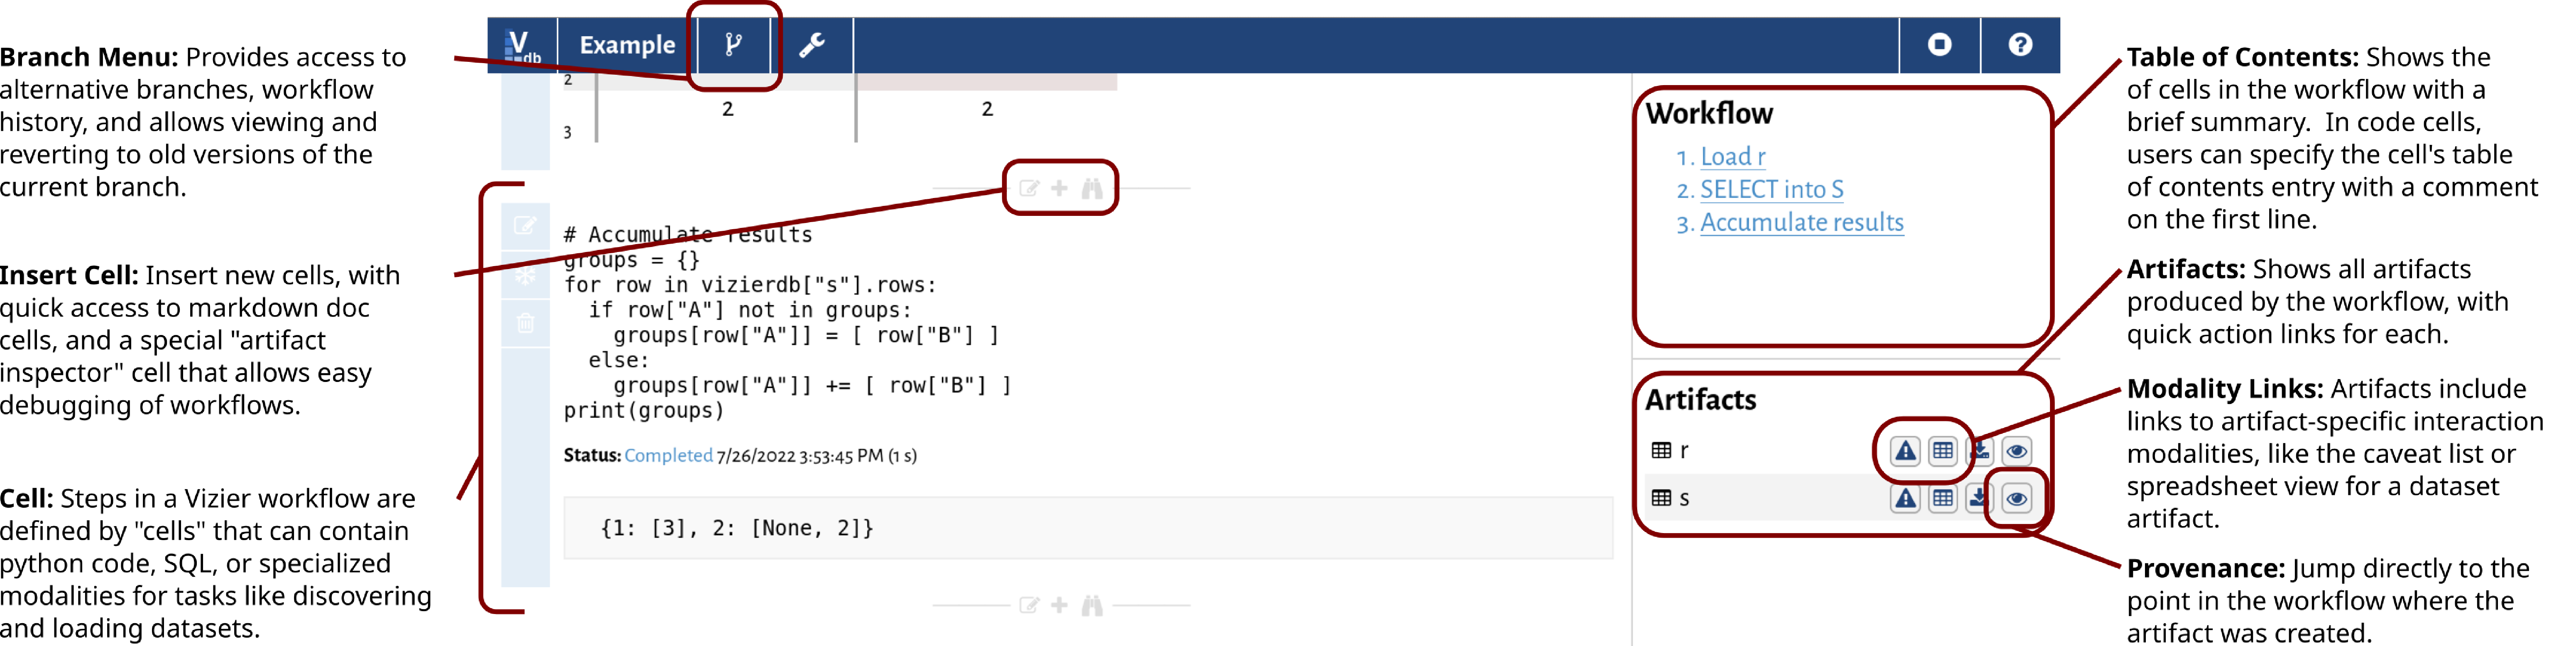
\includegraphics[width=\textwidth]{graphics/screenshot.pdf} 
  \caption{The Vizier User Interface}
  \label{fig:screenshot}
\end{figure}
%%%%%%%%%%%%%%%%%%%%%%%%%%%%%%%%%%%%%%%%%%%%%%%%%%%%%%%%%%%%%%%%%%%%%%%%%%%%%%%%

%%% Local Variables:
%%% mode: latex
%%% TeX-master: "../2022_IEEE_DEB_Vizier"
%%% End:


\section{Overview of proposed solution}

%In our work, we have built a proof-of-concept system that enhances the internal 
%reasoning in the operating system and its computation of resource allocation 
%policies by taking into account the workload properties, as well as enabling 
%for a richer information flow with the database layer. We also revisited the generic 
%OS services and mechanisms and adapted them to better suit the requirements of 
%modern data processing workloads, integrating them as part of a novel OS architecture.

More specifically, we propose customizing the operating system for data-processing applications
and enriching the interface between the two layers to allow for better information flow.
This way the operating system can adjust its allocation policies while reasoning about 
the workload requirements in addition to its optimization for system-wide objectives.
To achieve that, we built a proof-of-concept system that makes the following contributions:

First, we show how the semantic gap between data processing engines and the 
operating system can be avoided by introducing a declarative interface for mutual information
exchange. To do that we explored how to best integrate some of the extensive knowledge 
that a database engine has about its workload requirements (e.g., cost models, data 
dependency graphs, resource requirements, etc.) into the OS. The goal is to enable 
the OS to reason both about the particular requirements and properties of the database 
and about the system-wide and runtime view of the hardware platform and the current
application mix. We achieve that by introducing a policy engine in the OS and a 
resource monitor that facilitates the communication between the two layers. 
A rich \textit{query-based interface} 
then enables any application (including the database) to interact with the policy 
engine. More specifically, it allows the database to (i) query for details about the 
underlying hardware resources, (ii) rely on the policy engine to absorb the hardware 
complexity and diversity, and provide suitable deployment decisions, and (iii) 
push database-specific logic down to the OS in the form of stored procedures that 
enables it to adjust and react to noisy system environments (\S~\ref{sec:policy}). 
The system architecture is shown in Figure~\ref{fig:policy_engine}. 


Second, inspired by the multikernel OS design~\cite{baumann:sosp09}, in \S~\ref{sec:basslet}
we propose a novel OS architecture that enables dynamic partitioning of the 
machine's resources (e.g., CPUs, memory controllers, accelerators, etc.) into a 
\textit{control plane}, running a full-weight operating system along with an OS 
policy engine, and a \textit{compute plane}, consisting of specialized light-weight 
OS stacks. The objective is to enable customization of the compute-plane OS both 
for the properties of the underlying hardware (i.e., potentially heterogeneous
compute units) and for the specific requirements of the workload (e.g., customized 
scheduler or memory management). By design the allocation of resources between the 
control and compute plane is dynamic and can be adapted at runtime based on the 
changing workload requirements. 
To demonstrate the benefits of such control-compute plane OS architecture, we present 
a light-weight OS with a kernel-integrated runtime (Basslet), which we run on the 
compute plane, that is customized for parallel data analytics. 

% \input{policy}

\section{OS policy engine}
\label{sec:policy}

The OS policy engine is designed to enable both the OS itself and the database running on top
to better grasp the properties of the available hardware resources and reason about the 
real-time system state. 

\begin{figure}
  \centering
  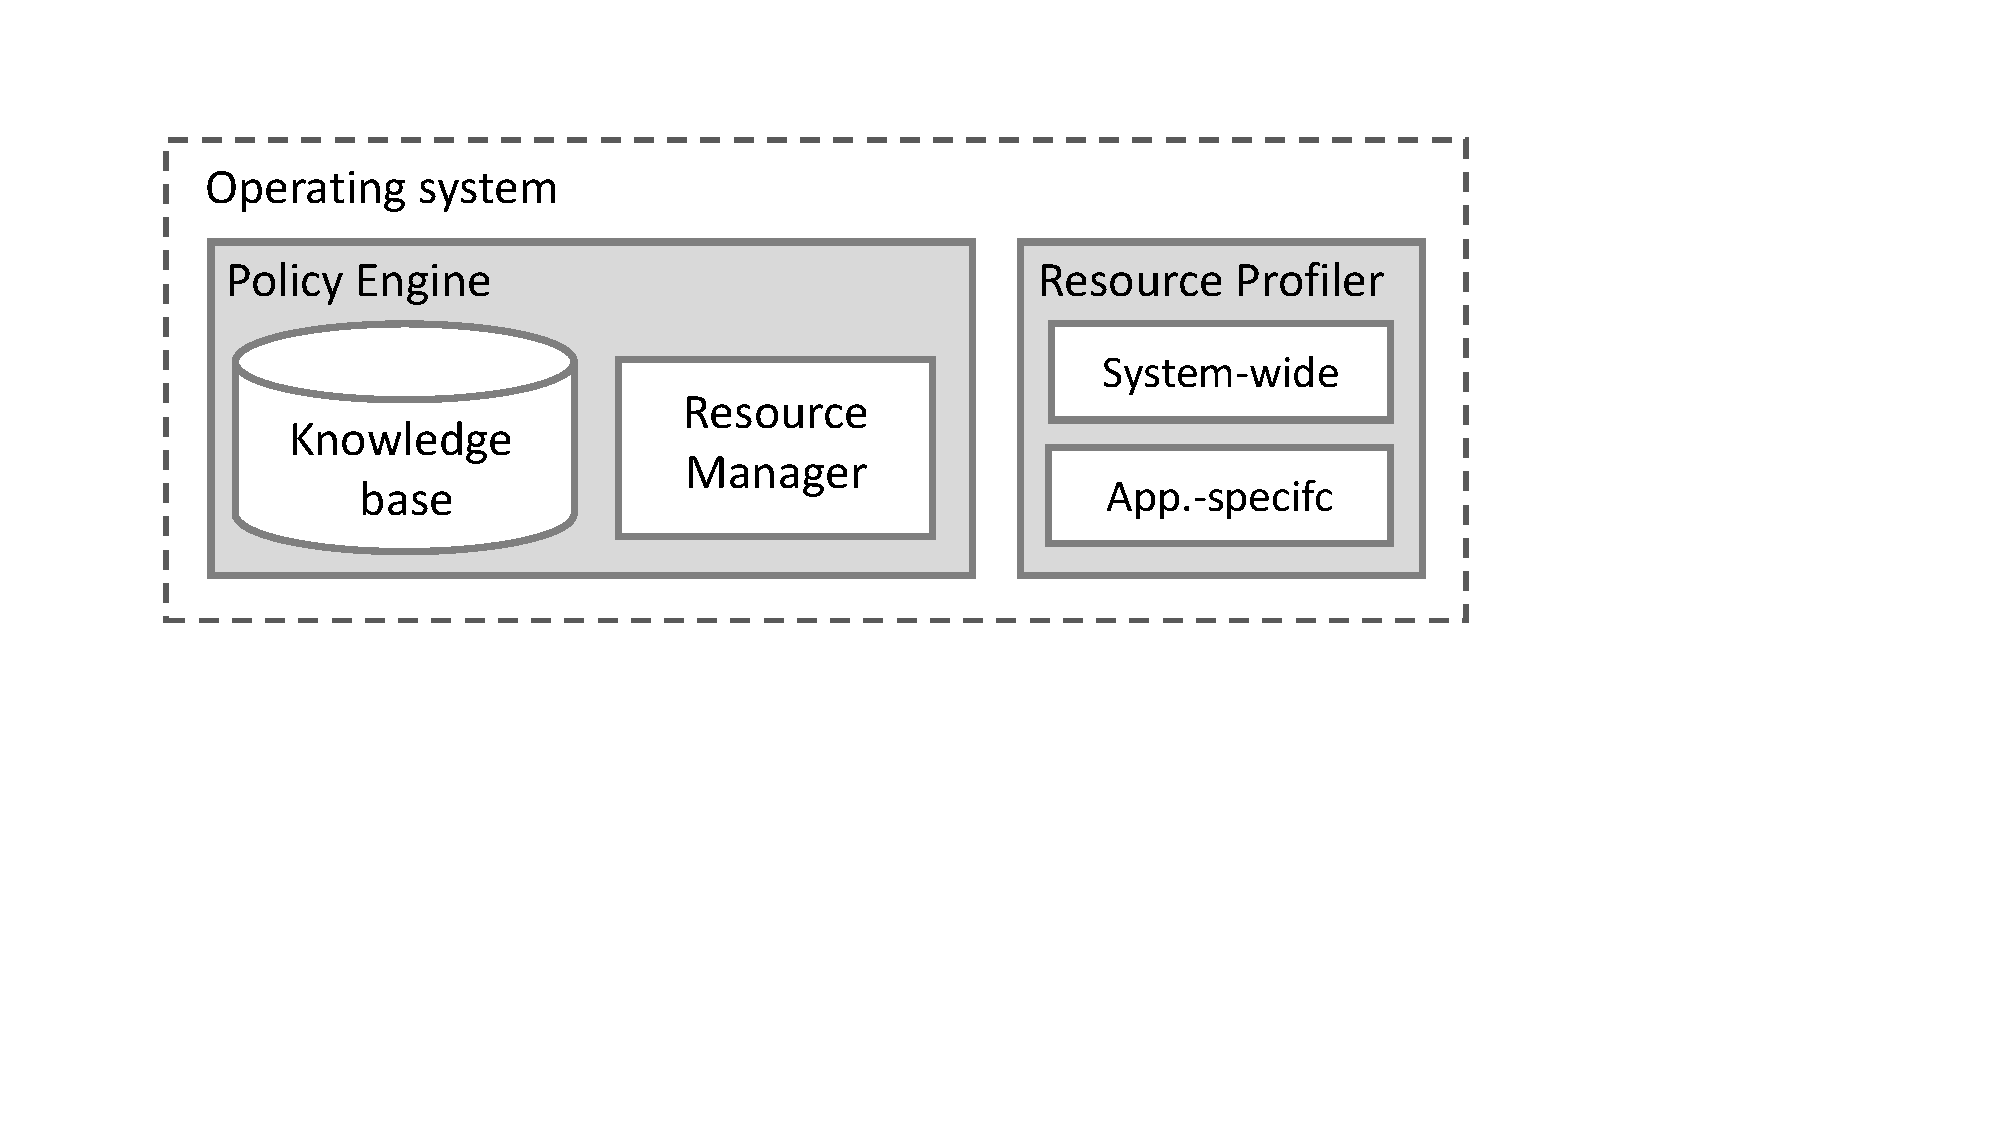
\includegraphics[scale=0.6, trim=2cm 8cm 8cm 2cm, clip=true]
    {figs/intro_policyengine}
  \caption{Policy Engine}
  \label{fig:policy_engine}
\end{figure}

More specifically, it consists of a \textit{knowledge base} that contains
information about (1) machine specific facts (e.g., topology of the machine, number of cores and
memory per NUMA node, the cache hierarchy, etc.), (2) application-related facts
(e.g., information whether an application is compute- or memory-bound, sensitive to sharing 
the caches, etc.), and (3) current system-state (e.g., number of active applications, 
their memory usage, etc.). This information is used both by the knowledge base to build
a detailed model of the machine and its resources, and by a set of algorithms and solvers
that compute resource allocation schedules. 
For the knowledge base we borrow and extend the concept of System Knowledge Base (SKB) 
from the Barrelfish OS~\cite{Schuepbach12, barrelfish}, which stores data in the format of
free-form predicates in a Constraint Logic Programming (CLP) engine. This enables various 
solvers to reason about the information available by issuing logical queries to perform 
constraint solving and optimization.

The \textit{resource manager} is responsible for communicating with the applications (in our 
case the database engine), triggering resource allocation computations in the knowledge base,
and executing the decided policies by invoking the available OS mechanisms. 
Often, the policy engine relies on a \textit{resource profiler} to measure the capacities 
of hardware resources (e.g., the maximum attainable DRAM bandwidth achievable per NUMA node), 
monitor their current utilization, and enable applications to measure their resource 
requirements or footprints.

Finally, the new {\it interface} is declarative and allows for richer two-way information exchange 
between the DBMS and the OS policy engine. It covers a wide range of actions from retrieving 
information about the underlying architecture to pushing down application-specific cost-models
and dataflow dependencies so that the OS policy engine can reason about them. Furthermore,
by allowing stored procedures it enables database-specific logic to be computed in 
the OS-side that leverages the most up-to-date system-state. Finally, it supports the 
retrieval of application-specific resource usage profiles as measured by the resource 
profiler and enables a continuous information flow between the two layers at runtime
in the form of notifications and updates. This way the OS can do a better job when 
deploying the application's threads onto a range of different machines and provide 
efficient resource allocation without affecting the application's performance of 
predictability; and the database can adapt itself based on the current system state,
which is especially important in noisy environments. 

%\subsection*{Implementation details}
%For the {\it knowledge base} we borrow and extend the concept of System Knowledge Base (SKB) 
%from the Barrelfish OS~\cite{Schuepbach12, barrelfish}. The SKB stores data in the format of
%free-form predicates in the Constraint Logic Programming (CLP) engine. This enables various 
%solvers to reason about the information available by issuing logical queries to perform 
%constraint solving and optimization. We augmented the knowledge stored in the SKB so that 
%it can be classified into two categories: 
%\begin{enumerate}
%\item {\it system-level facts} -- information about the underlying hardware platform (via resource 
%discovery at runtime and online micro-benchmarks) and the system state (via book-keeping of the
%running tasks and their resource usage/assignment), and 
%\item {\it application-specific facts} -- information about the application itself. 
%For instance, either application's properties that an OS can easily understand 
%(e.g., CPU-bound, maximum degree of parallelism, etc.) or that are specific to 
%the application's domain (e.g., dataset size, latency SLOs, etc.). The latter type 
%can only be leveraged by application-specific \textit{stored procedures} that 
%compute system-level properties (e.g., minimum number of cores).
%\end{enumerate}
%As such the SKB is the reactive component of the policy engine that can be seen as a 
%repository and a calculation engine for system knowledge. It is complemented by the
%{\it resource manager}, which is the active component that triggers re-computation of the 
%resource allocation as soon as a new task enters and registers in the system. It is also 
%responsible for implementing the resulting OS policy using the available OS mechanisms. 
%
%The {\it interface} between the database engine and the OS policy engine provides support 
%for knowledge exchange that covers a range of actions from retrieving information about 
%the underlying architecture to pushing down application-specific cost-models and 
%dataflow dependencies so that the OS policy engine can reason about them. Furthermore,
%by allowing stored procedures it enables database-specific logic to be computed in 
%the OS-side that leverages the most up-to-date system-state. Finally, it supports the 
%retrieval of application-specific resource usage profiles as measured by the resource 
%profiler and enables a continuous information flow between the two layers at runtime
%in the form of notifications and updates.

\subsection*{Examples}
We demonstrate the benefits of the policy engine and importance of leveraging unified knowledge
from both the database engine and the operating system with two different examples.

\subsubsection*{Use-case 1: Adaptability to noisy environments}
In the first use-case we show how a storage engine (that we call CSCS) can be adjusted to 
interact more closely 
with the OS policy engine to achieve good performance and maintain predictable runtime even
in dynamic environment where other applications enter the system and begin using 
resources~\cite{cod:2013}.
Before starting the execution, the storage engine communicates with the policy engine its 
properties (i.e., its scan threads are CPU-bound, cache- and NUMA-sensitive, the SLO 
for latency is 3ms, etc.), a cost 
function that calculates the scan time given the specific workload properties on a 
particular machine, and a stored procedure for data redistribution among the remaining 
scan threads whenever a CPU core resource is revoked at the expense of a newly entered 
task in the system.

\begin{figure}
\begin{minipage}[b]{.5\linewidth}
\centering 
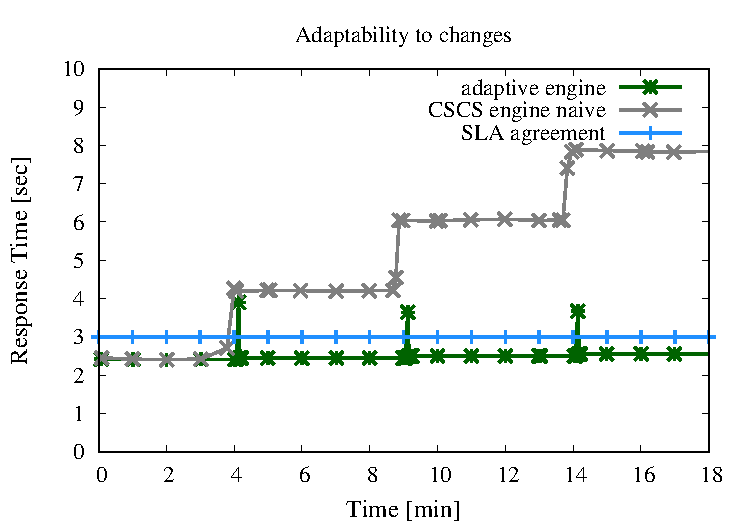
\includegraphics[width=\textwidth]{figs/adaptability_results}
\subcaption{Adaptability to noisy envirnonments}
\label{fig:1a}
\end{minipage}%
\begin{minipage}[b]{.5\linewidth}
\centering
%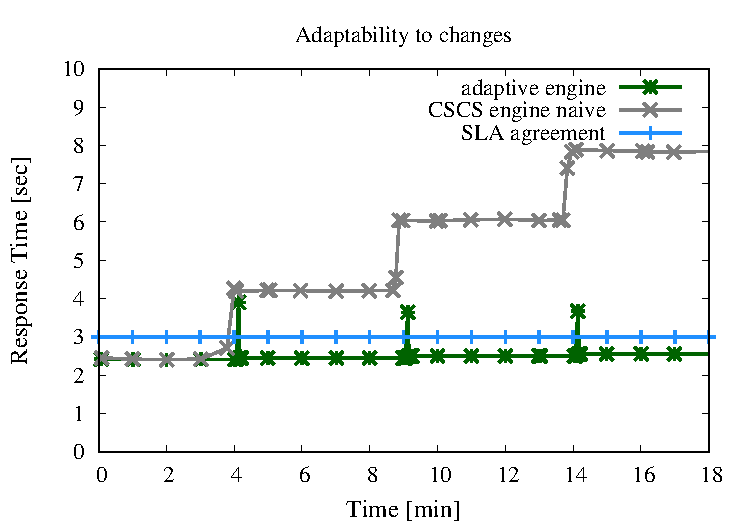
\includegraphics[width=\textwidth]{figs/adaptability_results}
  \centerline{\small
    \begin{tabular} {r r r r r r} 
    \hline \hline
    Scheduler& CPUs & Tput    & \multicolumn{3}{c}{Response Time[s]}          \\ 
             &       & [WIPS] & 50th   & 90th   & 99th    \\ \hline
    Depl Alg.& 6     & 428    & 15  & 23  & 36   \\
    SharedDB & 44    & 425    & 14  & 22  & 36   \\ 
    Linux    & 48    & 317    &  8  & 72  & 82   \\ 
    \hline \hline \vspace{1cm}
  \end{tabular}
  } 
  \subcaption{Deployment of complex query plan}
\label{fig:1b}
\end{minipage}
\end{figure}

When a new task enters the system it registers with the resource manager and asks for a CPU core.
The resource manager notifies the knowledge base of the new changes and triggers
a re-computation of the resource allocation plan. In this re-computation the policy engine
checks that even if it takes away a core from the storage engine, the scan time is still 
going to be below the 
runtime SLO and allocates one of the cores to the new application. The database storage engine 
is notified of the change and invokes the stored procedure to decide how to redistribute the
data that was scanned by the thread that just lost its CPU core. The stored procedure retrieves
information about the remaining available cores and checks the availability of memory on the 
corresponding NUMA nodes. It then redistributes the data to the chosen threads and resumes execution.
In Fig.~\ref{fig:1a} we compare the behaviour of a naive CSCS storage engine that does not 
react to changes in the system state and continues executing as if nothing happened (despite 
another CPU-intensive task entering the system every 4 minutes and pinning its thread
to core 0 where a scan thread runs) leading to significant reduction in response time. The 
adaptive-engine line shows how the storage engine behaves when coordinating with the 
policy engine. Its response time remains relatively steady even in the presence of 
other tasks with spikes observed at the time when a new task enters the system. 
We explain the spikes as a result of the storage engine redistributing the data to the 
other cores, as suggested by the stored procedure. Nevertheless, even when losing a scan 
thread (core), the storage engine can easily resume executing with a latency well within the 
required SLA requirements.

\subsubsection*{Use-case 2: Efficient deployment on multicore machine}

The second use-case demonstrates the benefits of using (1) the {\it resource profiler} to 
capture the resource requirements of database operations, (2) the {\it OS policy engine}
and its
knowledge of the underlying machine model and (3) the {\it DB engine}'s knowledge of the 
data-dependency graph between relational operators in a complex query plan, to compute 
a close to optimal deployment of the query plan on a given multicore 
machine~\cite{Giceva:vldb14}.

Good resource management and relational operator deployment requires awareness of 
the thread's resource requirements~\cite{Ailamaki:vldb99, manegold:vldb00, li2013numa}. 
As a result of tuning the algorithm's implementation to the underlying hardware, 
databases have also become more sensitive to the resources they have at hand and 
poor scheduling can lead to performance degradation~\cite{Lee:2009,cod:2013}.
In order to capture the relevant characteristics for application threads, the resource monitor
generates so-called {\it resource activity vectors} (RAVs). At present, they capture the usage 
of the most important resources (CPU and memory bandwidth usage), but can be easily extended to 
other resources when needed (e.g., network I/O utilization, cache sensitivity, etc.).
The approach was inspired by the notion of activity vectors, initially proposed for 
energy-efficient scheduling on multicore machines~\cite{merkel2010}.

The deployment algorithm for a given query plan runs in the OS policy engine and aims to 
minimize the computational- and bandwidth- requirements for the query plan, provide NUMA-aware
deployment of the relational operators and enhance data-locality. As input, it uses (1) the 
data-dependency graph of the relational operators as provided by the database engine, (2)
the RAVs for each operator as generated by the resource monitor, and (3) a detailed model of 
the underlying machine as kept in the OS policy engine. 
The algorithm consists of four phases, where the first two compute the required number of
cores (corresponding to the {\it temporal scheduling} sub-problem), the third phase 
approximates the minimum number of required NUMA nodes and the fourth phase computes
the final placement of the cores on the machine so that it minimizes DRAM bandwidth usage
-- the {\it spatial scheduling} sub-problem.

We evaluated the effectiveness of the algorithm by deploying a TPC-W global query plan as 
generated by SharedDB~\cite{SharedDB} (with 44 relational operators) on the AMD 
Magnycore machine (four 2.2~GHz AMD 
Opteron 6174 processors and 128~GB RAM, each processor has two 6-core dies, or 48 cores
in total). We compare the performance of running the workload
against two baselines: (1) using the default Linux scheduler and (2) using the standard 
operator-per-core deployment used by systems like SharedDB to provide guarantees for
predictable performance and tail latencies. The results are shown in Tab.~\ref{fig:1b}. 
The presented values for average throughput and latency percentiles (50th, 90th, and 99th) 
show that the performance of the system was not compromised by the significant 
reduction in allocated resources (44 for SharedDB default scheduler down to 6 cores for 
our algorithm), which is important for databases and their SLOs. Please note that the 
performance of the query plan when the Linux scheduler was in charge of the deployment
is poorer in both absolute throughput performance and stability than the other two 
approaches. This is because the OS can use all 48 cores on the machine and often migrates 
threads around based on some system-wide metric which leads to higher tail latencies.

%\input{basslet}

\section{Customized OS}
\label{sec:basslet}
%Second,
%we propose a novel OS architecture that enables dynamic partitioning of the machine's resources
%(e.g., CPUs, memory controllers, accelerators, etc.) into a \textit{control plane}, running a full-weight
%operating system stack and the OS policy engine, and a \textit{compute plane}, consisting of 
%specialized light-weight OS stack. The main goal is to allow customization of the OS stack both for
%the properties of the underlying hardware (i.e., potentially heterogeneous compute units) and the 
%specific requirements of the workload running on top (e.g., customized execution or memory model). 
%To demonstrate its benefits we present a light-weight OS stack (kernel, runtime and selected 
%library OS services) that we customized for running parallel data analytics. The allocation of resources
%between the control and compute plane is dynamic and can be adapted at runtime based on the changing
%workload requirements. 

In the previous section we showed the benefits of using the unified knowledge from 
both the DB engine and the OS policy engine. While the design can bring significant advantages 
in a noisy environment and when scheduling jobs on a multicore system, it still does not alter
the fact that the resource manager of the OS policy engine needs to use the full-blown OS s
tack with all of its generic mechanisms. 
Recent advancements in operating system design enable us to
configure and specialize the OS system stack (i.e., apply changes in both kernel- and user-space)
for particular workload classes. Some new operating systems are based on the multikernel
design~\cite{baumann:sosp09}, which run a separate kernel on every 
core~\cite{barrelfish,fos:osr09,Chapin:sosp95}. In the Barrelfish OS the state on each core is 
(relatively) decoupled from the rest of the system -- a multikernel can run multiple different 
kernels on different cores~\cite{zellweger:osdi14}.

\subsection{Novel OS architecture and the case for customized kernels}

The novel OS architecture (Badis) we propose leverages the flexibility of the Barrelfish multikernel 
design that enables us to have an optimized lightweight OS co-exist in the same system as 
other general purpose OS kernels. We show the design in Fig.~\ref{fig:basslet}. In a nutshell, Badis
splits the machine's resources into a {\it control plane} and a {\it compute plane}. The control 
plane runs the full-weight OS stack (FWK), while the compute plane consists of customized lightweight
kernels (LWKs). The compute plane kernels provide selected OS services tailored to a particular 
workload and a noise-free environment for executing jobs on behalf of applications whose main threads run on the control plane's FWK. Additionally, as we discuss later, Badis' modular design makes it suitable 
to address HW heterogeneity and enables OS customization for different compute resources.

\begin{figure}
  \centering
  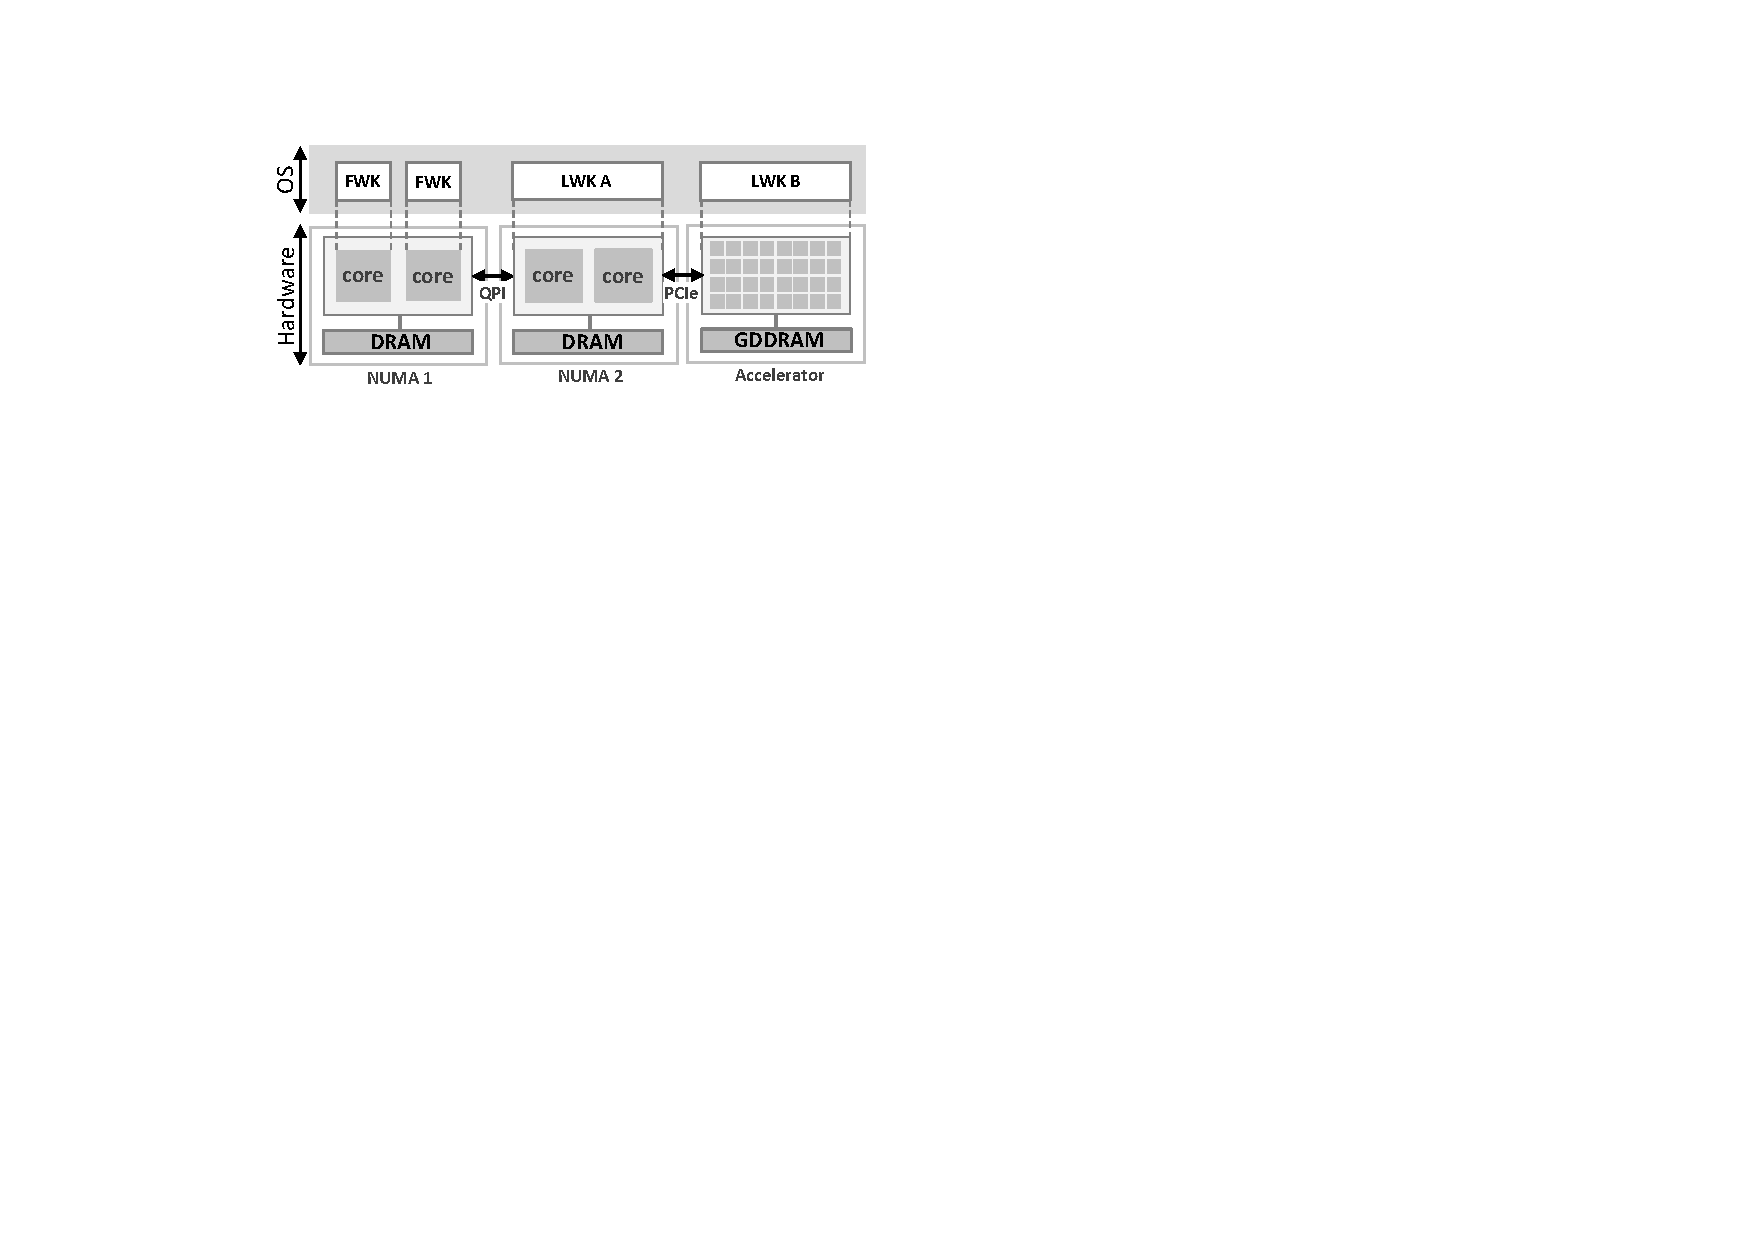
\includegraphics[trim=4cm 14cm 14cm 2.5cm, clip=true]
    {figs/multi-kernel}
  \caption{Illustrating Badis -- an adaptive OS architecture, based on the multikernel model.
  The cores on NUMA node 1 each execute a separate kernel of the full-weight kernel (FWK). The 
  cores on NUMA node 2 execute a common instance of a specialized light-weight kernel (LWK A).
  The computation units on the HW accelerator run a different version of the light-weight 
  kernel -- optimized for the particular hardware platform (LWK B).
  }
  \label{fig:basslet}
\end{figure}

To demonstrate the benefits, we designed and implemented a customized OS stack for 
executing parallel analytical workloads. Even though, in our work we identified 
multiple opportunities for improvement of resource management and scheduling 
(e.g., for CPUs, memory, and various hardware devices)~\cite{Giceva:damon16}, 
in the first prototype we focused primarily on managing CPU resources. 
More specifically, for parallel analytical workloads we identified the following requirements:
\begin{itemize}
 \item The need for {\it run-to-completion} tasks, which is important for both 
 synchronization-heavy workloads, where preemption can lead to the well-know 
 convoy effect~\cite{Blasgen:1979}, and data-intensive jobs that are 
 cache-sensitive, where preemption can often lead to cache pollution and 
 expensive DRAM accesses. In one of our experiments, we measured the indirect 
 cost of a context-switch on machines with large last-level caches to be as 
 expensive as 6ms, which is equivalent to the quantum on modern Linux schedulers.
 \item The need for {\it co-scheduling} for a group of threads that work on the same
 operation and especially for data processing workloads that have synchronization
 steps where a single straggler can impact performance.
 \item The need for {\it spatial isolation}. In particular, when running in a noisy
 environment alongside other application threads which also use the memory 
 subsystem. Such interaction can often result in destructive resource 
 sharing~\cite{Lee:2009, tang:isca11}. Hence, we claim that there is more to 
 allocation than just cores and one should also account for other resources such as
 shared caches and DRAM bandwidth. Given the properties of modern multicore machines
 one such hardware island~\cite{Porobic:vldb12} is a NUMA node. 
\end{itemize}

\subsection{Implementation and evaluation}

To achieve those requirements in the customized OS kernel, we proposed extending 
the UNIX-based process model to also support OS task and ptask (parallel task) 
as program execution units. This way the database can explicitly specify that a 
job needs to be executed without preemption -- OS task, or that a pool of 
user-level threads that execute a common parallel job should be co-scheduled 
until completion -- OS ptask. 
We implemented it as part of a kernel-based runtime, which can execute 
parallel analytical jobs on behalf of the data processing engine. Each customized
kernel is spawned on a separate NUMA node (hardware island) for spatial isolation.
As per design, the light-weight kernels run on the compute plane, while the
FWK on the control plane offers a traditional thread-based scheduling. The boundary 
between the two planes, as well as the type of compute-plane kernels, can be changed 
at runtime depending on the workload mix requirements. Note that the cost of switching a
kernel is as expensive as a context switch~\cite{zellweger:osdi14}. 
Such a dynamic architecture makes the system's stack suitable for scheduling 
hybrid workloads (e.g., operational analytics), where different kernels can 
co-exist at the same time, each one customized for a particular workload.

\begin{figure}[t]
\centering
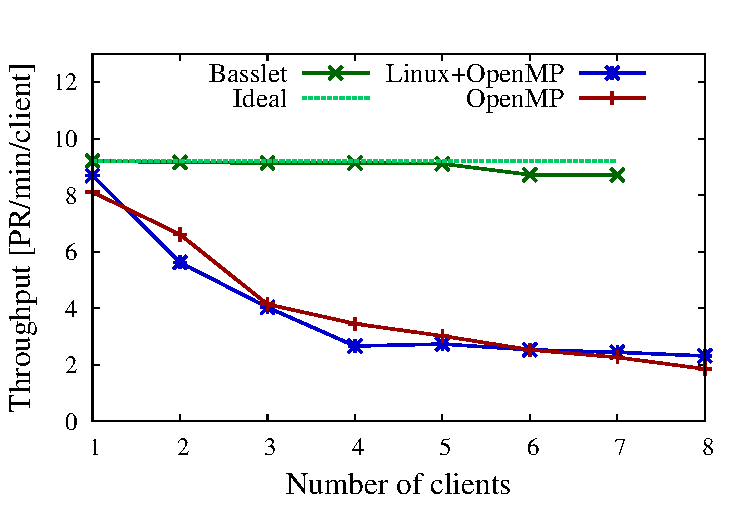
\includegraphics[width=0.55\textwidth]{figs/PR_scale_out.pdf}
\caption[Comparing throughput scale-out using OpenMP vs. 
Linux+OpenMP vs. \Runtime]
{Throughput scale-out when executing multiple \texttt{PR}s
using internal OpenMP parallelism vs. Linux+OpenMP scheduler 
vs. kernel-integrated runtime, as compared to ideal scale-out.}
\label{fig:basslet_results}
\end{figure}

To demonstrate that not only database engines can benefit from such a customized kernel
integrated runtime, we evaluated the system with GreenMarl~\cite{hong:asplos12}, a
graph application suite running on OpenMP. More specifically, we execute PageRank (PR) on the LiveJournal 
graph, which is the largest available social graph from the SNAP dataset~\cite{snapnets}. 
The experiment evaluates the efficiency of using the customized compute plane kernel 
compared to the performance of the same workload, when executed using either the 
default OpenMP or the Linux scheduler. All experiments were ran on the same 
AMD Magnycours machine as before. The workload is as follows: we measure the 
performance when a single client runs a PageRank algorithm on one NUMA node -- 
6 cores. For every subsequent client (i.e., another instance of PR) we allow
the system to use additional 6 cores of another NUMA node. The response variable
is the throughput as perceived per client (i.e., the inverse of the total time
needed to execute all PR jobs). The results are presented in Fig.~\ref{fig:basslet_results}.
They show that the interference among the clients when OpenMP or OpenMP+Linux 
schedule the resources, increases as we add more clients despite having sufficient
resources (there are 8 NUMA nodes and at most 8 PRs running in the system). 
In contrast, when using the kernel integrated runtime we can achieve almost linear 
per-client throughput scale-out until seven clients. The final six cores, belonging 
to the first NUMA node, are dedicated for the control plane.

While the discussion here focused on managing CPU resources for analytical
workloads, in \cite{Giceva:damon16} we also discuss opportunities for managing 
memory as well as providing more transparent access to other devices.

\subsection{Related work}
The HPC community has long argued that their workloads are
sensitive to OS ``noise'' when working at large scale~\cite{Hoefler:2010}.
Thus, they proposed using light-weight kernels~\cite{Riesen:2015,Kelly05,
Giampapa:2010} that are customized for sensitive applications. 
Researchers have also explored the design space of multikernel-based OSes by having the 
specialized light-weight kernels run alongside full-weight kernels like Linux inside the 
same system~\cite{FusedOS,mOS,Gerofi:2015}.

While our prototype is implemented over a multikernel, customized new schedulers can
be applied on Linux if we leverage some recent proposals for fast core 
reconfigurability~\cite{panneerselvam:atc15}. Currently, in our work we have not directly addressed I/O
issues, but the architecture allows to easily integrate the control/data plane 
ideas proposed by systems like Arrakis~\cite{Peter:osdi14} and IX~\cite{IX}. Similar 
approaches were also explored in Solros~\cite{solros} for workloads with high disk 
and network bandwidth requirements when running on co-processors.

% \input{challenges}

\section{Future outlook and research directions}

In this section, we look at recent and future developments of hardware technologies 
and deployment trends. We argue for a holistic solution across the system stack 
(from the data processing layer, down to runtime and operating systems and eventually 
hardware) in order to efficiently address the coming challenges and hide the 
increasing complexity from the developer's side.

\begin{figure}[t]
\centering
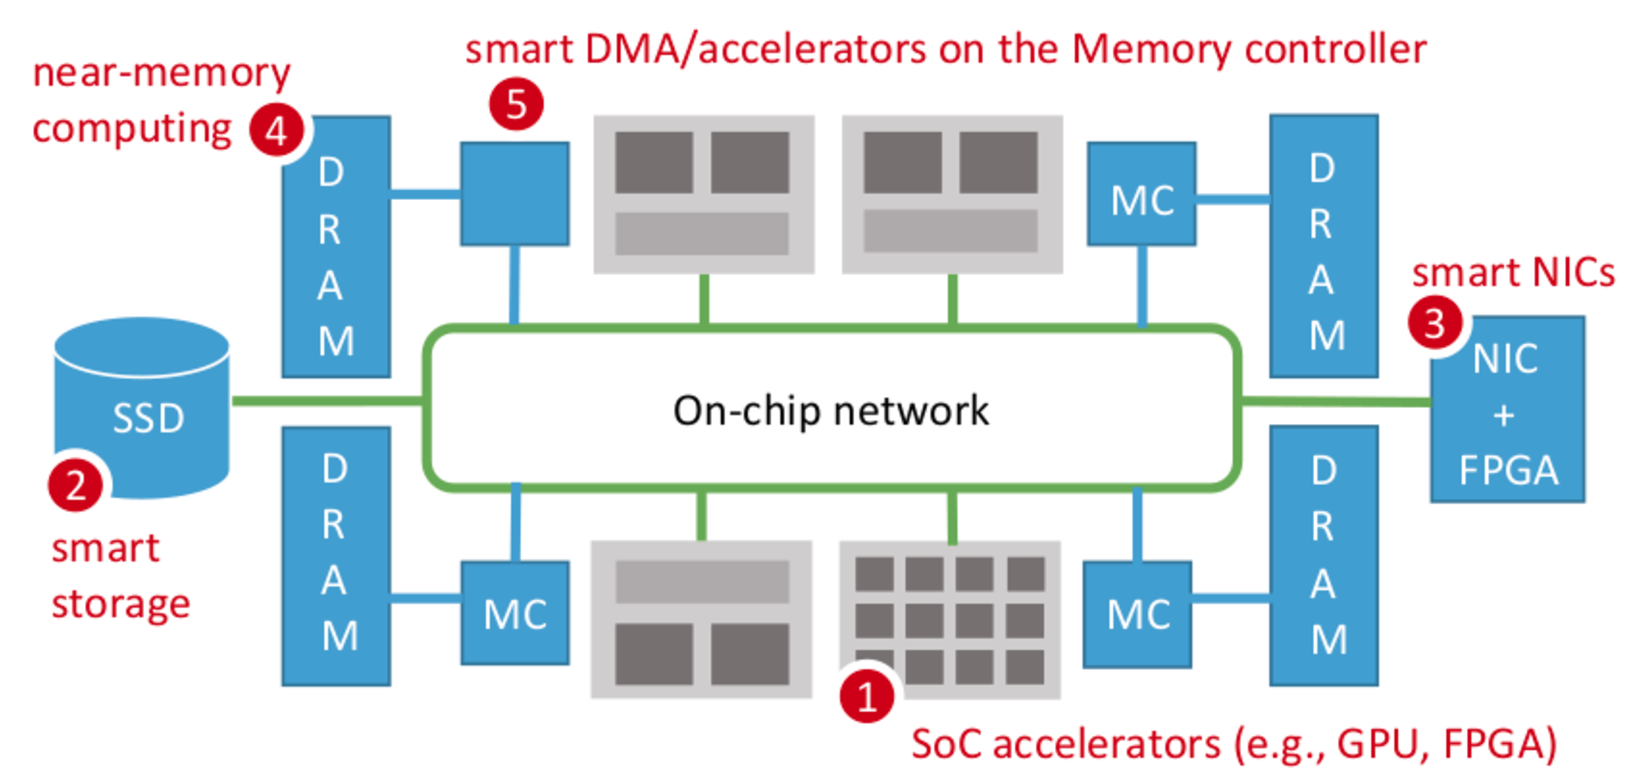
\includegraphics[width=0.7\textwidth]{figs/active-hw-everywhere-crop.pdf}
\caption{Active heterogeneous hardware}
\label{fig:active_hw}
\end{figure}

Modern machines have an abundance of hardware heterogeneity and they are only going to get 
more diverse. In Fig.~\ref{fig:active_hw} we show all the places where {\it active hardware}
components can be found today in addition to the regular CPUs: (1) system-on-chip 
accelerators like GPUs and FPGAs, (2) smart storage mediums (e.g., smart SSDs), 
(3) programmable NICs or NICs with an FPGA attached, as bump in the wire, 
offloading compute (4) to where the data sits (e.g., near-memory 
computing~\cite{PIM}) or (5) as the data moves between DRAM and the 
processor's cache (e.g., accelerators on the memory controller~\cite{aingaran2015m7}), etc.

Despite this outlook, today's commodity operating systems still hide the underlying 
hardware complexity and diversity as much as possible from the applications running above. 
While this made sense in the past, such an approach today is very restrictive and leads
to under-utilization of the available hardware capacity. We argue that the Badis OS
architecture is well-suited for such hardware platforms -- as opposed to 
treating all the active components as devices with external drivers (as with 
GPGPUs~\cite{Rossbach:2011} or NICs~\cite{Peter:osdi14,IX}), we should have the
OS manage their computational capacities in the {\it control plane} and export the 
device services directly to the applications via customized {\it compute
planes}~\cite{daniel}. Recent work in the OS community has also proposed extending 
the multikernel model for heterogeneous computing~\cite{legoos} and building 
data-centric OSs for accelerators~\cite{solros}.

Furthermore, it is important to note that the declarative interface between 
databases and operating systems becomes even more relevant in the case of hardware
heterogeneity. Especially when a data-processing engine can offload part of the 
computation to an active compute component. Constructing cost-models that match the 
performance/cost metrics for using an accelerator and pushing down such information
to the OS policy engine, can make the scheduling and resource management of these 
resources much more effective. If this is also accompanied with the data-dependency
graph as we have shown for other hybrid systems~\cite{daniel}, the underlying OS can
absorb the complexity of memory management and task allocation on behalf of the 
developer and achieve much higher performance and more efficient resource usage.

Going beyond database engines, many machine learning, data mining and 
graph processing applications can benefit from similar cross-layer optimizations across 
the systems stack, including the operating system. We are currently exploring
how such workloads can benefit by sharing information about their cost models or 
dataflow graphs to the OS policy engine when executing on heterogeneous
computing platforms (e.g., TPUs or FPGAs). 

%\vspace{-.5cm}
\section{Conclusion}
\label{sec:conclusion}

Online job platforms are becoming increasingly popular.
They provide an alternative job arrangement that has the potential to dramatically affect the Future of Work. 
An increasing proportion of human workforce will be employed in such platforms.
Hence, it is very important to study the problem of platform design.
In this paper, we have a preliminary attempt at investigating this problem.
We provide a taxonomy of platforms and what are the major missing functionalities for both workers and requesters. 
We also advocate the need for interoperability between platforms.
This allows workers and requesters to move their data between platforms without getting locked into a single platform. 
There are a number of interesting research and policy challenges in achieving the vision of platform interoperability.


\section{Conclusion}

The interaction between database engines and operating systems has been a difficult
problem for decades, as both try to control and manage the same resources but with
different goals. For long time, databases had the luxury to ignore the OS and 
overwrite the generic policies thanks to hardware homogeneity and over-provisioning 
of resources (i.e., running a database alone on a dedicated server machine).
With the latest trends in hardware development (e.g.,from multicore to various 
accelerators) and workload deployment (e.g., multi-tenancy and server consolidation 
in the cloud), these assumptions are no longer valid. Hence, we argue that 
{\it now} is the time for a holistic approach that crosses multiple layers of 
the system stack and in particular one that revisits the interface between 
database management and operating systems. 

In this article, as main problems we identified the knowledge gap that exists between
the two systems and the rigid interface that does not allow for richer information
flow as well as the generic policies offered by conventional operating systems for a 
wide range of applications. To address these issues we proposed Badis, an OS 
control- compute-plane architecture that allows for customization of the compute-plane
OS stack for a particular workload or underlying hardware platform, and a 
powerful OS policy engine that resides on the control plane, which is able to reason
about the database specific properties and requirements. With a series of experiments
we demonstrated the benefits of the approach of unifying the knowledge of the two
layers both for efficient deployment on modern machines and for maintenance of good 
and predictable performance in noisy environments. Looking forward, we believe that
the proposed design principles are going to become even more relevant in the context 
of active hardware and resource dis-aggregation, and extend beyond the requirements 
of traditional data management workloads.

\begin{thebibliography}{10}
\itemsep=1pt
\begin{small}

\bibitem{barrelfish}
{Barrelfish {O}perating {S}ystem}, 2019.
\newblock \url{www.barrelfish.org}, accessed 2019-01-20.

\bibitem{PIM}
J.~Ahn, S.~Yoo, O.~Mutlu, and K.~Choi.
\newblock {PIM-enabled Instructions: A Low-overhead, Locality-aware
  Processing-in-memory Architecture}.
\newblock In {\em ISCA '15}, pages 336--348, 2015.

\bibitem{Ailamaki:vldb99}
A.~Ailamaki, D.~J. DeWitt, M.~D. Hill, and D.~A. Wood.
\newblock {DBMSs on a Modern Processor: Where Does Time Go?}
\newblock In {\em VLDB~'99}, pages 266--277, 1999.

\bibitem{aingaran2015m7}
K.~Aingaran et~al.
\newblock M7: Oracle's next-generation sparc processor.
\newblock {\em IEEE Micro}, 35(2):36--45, 2015.

\bibitem{balkesen:15}
C.~Balkesen.
\newblock {\em In-memory parallel join processing on multi-core processors}.
\newblock PhD thesis, ETH Zurich, 2014.

\bibitem{baumann:sosp09}
A.~Baumann, P.~Barham, P.-E. Dagand, T.~Harris, R.~Isaacs, S.~Peter, T.~Roscoe,
  A.~Sch\"{u}pbach, and A.~Singhania.
\newblock {The multikernel: a new OS architecture for scalable multicore
  systems}.
\newblock In {\em SOSP}, pages 29--44, 2009.

\bibitem{IX}
A.~Belay, G.~Prekas, A.~Klimovic, S.~Grossman, C.~Kozyrakis, and E.~Bugnion.
\newblock {IX: A Protected Dataplane Operating System for High Throughput and
  Low Latency}.
\newblock OSDI'14, pages 49--65.

\bibitem{Blasgen:1979}
{Blasgen, Mike and Gray, Jim and Mitoma, Mike and Price, Tom}.
\newblock {The Convoy Phenomenon}.
\newblock {\em SIGOPS Oper. Syst. Rev.}, 13(2):20--25, 1979.

\bibitem{Chapin:sosp95}
J.~Chapin, M.~Rosenblum, S.~Devine, T.~Lahiri, D.~Teodosiu, and A.~Gupta.
\newblock {Hive: Fault Containment for Shared-memory Multiprocessors}.
\newblock In {\em SOSP}, pages 12--25, 1995.

\bibitem{daniel}
{Daniel Grumberg}.
\newblock {Customized OS kernel for data-processing on modern hardware}, 2018.

\bibitem{Gerofi:2015}
B.~Gerofi, M.~Takagi, Y.~Ishikawa, R.~Riesen, E.~Powers, and R.~W. Wisniewski.
\newblock {Exploring the Design Space of Combining Linux with Lightweight
  Kernels for Extreme Scale Computing}.
\newblock ROSS '15, pages 5:1--5:8, 2015.

\bibitem{Giampapa:2010}
M.~Giampapa, T.~Gooding, T.~Inglett, and R.~W. Wisniewski.
\newblock {Experiences with a Lightweight Supercomputer Kernel: Lessons Learned
  from Blue Gene's CNK}.
\newblock SC '10, pages 1--10, 2010.

\bibitem{SharedDB}
G.~Giannikis, G.~Alonso, and D.~Kossmann.
\newblock {SharedDB: killing one thousand queries with one stone}.
\newblock {\em VLDB}, 5(6):526--537, Feb. 2012.

\bibitem{Giceva:vldb14}
J.~Giceva, G.~Alonso, T.~Roscoe, and T.~Harris.
\newblock {Deployment of Query Plans on Multicores}.
\newblock {\em {PVLDB}}, 8(3):233--244, 2014.

\bibitem{cod:2013}
J.~Giceva, T.-I. Salomie, A.~Sch{\"u}pbach, G.~Alonso, and T.~Roscoe.
\newblock {COD: Database/Operating System Co-Design}.
\newblock In {\em CIDR~'13}, 2013.

\bibitem{Giceva:damon16}
J.~Giceva, G.~Zellweger, G.~Alonso, and T.~Rosco.
\newblock {Customized OS Support for Data-processing}.
\newblock In {\em The 12th International Workshop on Data Management on New
  Hardware}, pages 2:1--2:6, 2016.

\bibitem{Hoefler:2010}
T.~Hoefler, T.~Schneider, and A.~Lumsdaine.
\newblock {Characterizing the Influence of System Noise on Large-Scale
  Applications by Simulation}.
\newblock SC '10, pages 1--11, 2010.

\bibitem{hong:asplos12}
S.~Hong, H.~Chafi, E.~Sedlar, and K.~Olukotun.
\newblock {Green-Marl}: A {DSL} for easy and efficient graph analysis.
\newblock In {\em ASPLOS}, pages 349--362, 2012.

\bibitem{Shoal}
S.~Kaestle, R.~Achermann, T.~Roscoe, and T.~Harris.
\newblock {Shoal: Smart Allocation and Replication of Memory for Parallel
  Programs}.
\newblock In {\em Proceedings of the 2015 USENIX Conference on Usenix Annual
  Technical Conference}, USENIX ATC '15, pages 263--276, 2015.

\bibitem{Kelly05}
S.~M. Kelly and R.~Brightwell.
\newblock Software architecture of the light weight kernel, catamount.
\newblock In {\em In Cray User Group}, pages 16--19, 2005.

\bibitem{HyPer}
A.~Kemper and T.~Neumann.
\newblock {HyPer: A hybrid OLTP\&OLAP main memory database system based on
  virtual memory snapshots}.
\newblock In {\em ICDE}, pages 195--206, 2011.

\bibitem{Kimura:2015}
H.~Kimura.
\newblock {FOEDUS: OLTP Engine for a Thousand Cores and NVRAM}.
\newblock SIGMOD '15, pages 691--706, 2015.

\bibitem{Lee:2009}
R.~Lee, X.~Ding, F.~Chen, Q.~Lu, and X.~Zhang.
\newblock {MCC-DB: Minimizing Cache Conflicts in Multi-core Processors for
  Databases}.
\newblock {\em PVLDB}, 2(1):373--384, Aug. 2009.

\bibitem{Leis:sigmod14}
V.~Leis, P.~Boncz, A.~Kemper, and T.~Neumann.
\newblock {Morsel-driven Parallelism: A NUMA-aware Query Evaluation Framework
  for the Many-core Age}.
\newblock In {\em SIGMOD~'14}, pages 743--754.

\bibitem{snapnets}
J.~Leskovec and A.~Krevl.
\newblock {SNAP Datasets}: {Stanford} large network dataset collection.
\newblock \url{http://snap.stanford.edu/data}, June 2014.

\bibitem{li2013numa}
Y.~Li, I.~Pandis, R.~M{\"u}ller, V.~Raman, and G.~M. Lohman.
\newblock {NUMA-aware} algorithms: the case of data shuffling.
\newblock In {\em CIDR~'13}, 2013.

\bibitem{Lozi:eurosys16}
J.~Lozi, B.~Lepers, J.~R. Funston, F.~Gaud, V.~Qu{\'{e}}ma, and A.~Fedorova.
\newblock {The Linux scheduler: a decade of wasted cores}.
\newblock In {\em EuroSys'16}, page~1, 2016.

\bibitem{Makreshanski:vldb15}
D.~Makreshanski, J.~J. Levandoski, and R.~Stutsman.
\newblock {To Lock, Swap, or Elide: On the Interplay of Hardware Transactional
  Memory and Lock-Free Indexing}.
\newblock {\em {PVLDB}}, 8(11):1298--1309, 2015.

\bibitem{manegold:vldb00}
S.~Manegold, P.~A. Boncz, and M.~L. Kersten.
\newblock {Optimizing database architecture for the new bottleneck: memory
  access}.
\newblock {\em PVLDB~'00}, 9(3):231--246, 2000.

\bibitem{merkel2010}
A.~Merkel, J.~Stoess, and F.~Bellosa.
\newblock Resource-conscious scheduling for energy efficiency on multicore
  processors.
\newblock In {\em {EuroSys~'10}}, pages 153--166, 2010.

\bibitem{solros}
C.~Min, W.~Kang, M.~Kumar, S.~Kashyap, S.~Maass, H.~Jo, and T.~Kim.
\newblock {Solros: A Data-centric Operating System Architecture for
  Heterogeneous Computing}.
\newblock In {\em EuroSys}, pages 36:1--36:15, 2018.

\bibitem{muller:16}
I.~Mueller.
\newblock {\em Engineering Aggregation Operators for Relational In-memory
  Database Systems}.
\newblock PhD thesis, Karlsruhe Institute of Technology (KIT), 2016.

\bibitem{panneerselvam:atc15}
S.~Panneerselvam, M.~Swift, and N.~S. Kim.
\newblock {Bolt: Faster Reconfiguration in Operating Systems}.
\newblock In {\em 2015 USENIX Annual Technical Conference (USENIX ATC 15)},
  pages 511--516, Santa Clara, CA, July 2015. USENIX Association.

\bibitem{FusedOS}
Y.~Park, E.~Van~Hensbergen, M.~Hillenbrand, T.~Inglett, B.~Rosenburg, K.~D.
  Ryu, and R.~W. Wisniewski.
\newblock Fusedos: Fusing lwk performance with fwk functionality in a
  heterogeneous environment.
\newblock In {\em Proceedings of the 2012 IEEE 24th International Symposium on
  Computer Architecture and High Performance Computing}, SBAC-PAD '12, pages
  211--218, Washington, DC, USA, 2012. IEEE Computer Society.

\bibitem{Peter:osdi14}
S.~Peter, J.~Li, I.~Zhang, D.~R.~K. Ports, D.~Woos, A.~Krishnamurthy,
  T.~Anderson, and T.~Roscoe.
\newblock {Arrakis: The Operating System is the Control Plane}.
\newblock In {\em OSDI}, pages 1--16, 2014.

\bibitem{Polychroniou:2014}
O.~Polychroniou and K.~A. Ross.
\newblock {A Comprehensive Study of Main-memory Partitioning and Its
  Application to Large-scale Comparison- and Radix-sort}.
\newblock In {\em SIGMOD}, pages 755--766, 2014.

\bibitem{Porobic:icde14}
D.~Porobic, E.~Liarou, P.~Tozun, and A.~Ailamaki.
\newblock {ATraPos: Adaptive transaction processing on hardware Islands}.
\newblock In {\em ICDE~'14}, pages 688--699, 2014.

\bibitem{Porobic:vldb12}
D.~Porobic, I.~Pandis, M.~Branco, P.~Tozun, and A.~Ailamaki.
\newblock {OLTP on Hardware Islands}.
\newblock {\em PVLDB~'12}, 5(11):1447--1458.

\bibitem{Riesen:2015}
R.~Riesen, A.~B. Maccabe, B.~Gerofi, D.~N. Lombard, J.~J. Lange, K.~Pedretti,
  K.~Ferreira, M.~Lang, P.~Keppel, R.~W. Wisniewski, R.~Brightwell, T.~Inglett,
  Y.~Park, and Y.~Ishikawa.
\newblock {What is a Lightweight Kernel?}
\newblock ROSS '15, pages 9:1--9:8, 2015.

\bibitem{Rossbach:2011}
C.~J. Rossbach, J.~Currey, M.~Silberstein, B.~Ray, and E.~Witchel.
\newblock {PTask: Operating System Abstractions to Manage GPUs As Compute
  Devices}.
\newblock In {\em SOSP}, pages 233--248, 2011.

\bibitem{satish:sigmod10}
N.~Satish, C.~Kim, J.~Chhugani, A.~D. Nguyen, V.~W. Lee, D.~Kim, and P.~Dubey.
\newblock {Fast sort on CPUs and GPUs: a case for bandwidth oblivious SIMD
  sort}.
\newblock In {\em SIGMOD~'10}, pages 351--362, 2010.

\bibitem{Schuepbach12}
A.~Schuepbach.
\newblock {\em {Tackling OS Complexity with Declarative Techniques}}.
\newblock PhD thesis, ETHZ, Dec. 2012.

\bibitem{legoos}
Y.~Shan, Y.~Huang, Y.~Chen, and Y.~Zhang.
\newblock {LegoOS: A Disseminated, Distributed {OS} for Hardware Resource
  Disaggregation}.
\newblock In {\em {OSDI}}, pages 69--87, 2018.

\bibitem{Stonebraker:1981}
M.~Stonebraker.
\newblock {Operating System Support for Database Management}.
\newblock {\em Commun. ACM}, 24(7):412--418, July 1981.

\bibitem{tang:isca11}
L.~Tang, J.~Mars, N.~Vachharajani, R.~Hundt, and M.~L. Soffa.
\newblock {The Impact of Memory Subsystem Resource Sharing on Datacenter
  Applications}.
\newblock In {\em ISCA}, pages 283--294, 2011.

\bibitem{wassenberg2011}
J.~Wassenberg and P.~Sanders.
\newblock Engineering a multi-core radix sort.
\newblock In {\em Euro-Par 2011 Parallel Processing}, pages 160--169. Springer,
  2011.

\bibitem{fos:osr09}
D.~Wentzlaff and A.~Agarwal.
\newblock {Factored operating systems (fos): the case for a scalable operating
  system for multicores}.
\newblock {\em SIGOPS Operating Systems Review}, 43(2):76--85, 2009.

\bibitem{mOS}
R.~W. Wisniewski, T.~Inglett, P.~Keppel, R.~Murty, and R.~Riesen.
\newblock {mOS: An Architecture for Extreme-scale Operating Systems}.
\newblock ROSS '14, pages 2:1--2:8, 2014.

\bibitem{zellweger:osdi14}
G.~Zellweger, S.~Gerber, K.~Kourtis, and T.~Roscoe.
\newblock Decoupling cores, kernels, and operating systems.
\newblock In {\em OSDI}, pages 17--31, Oct. 2014.
 
\end{small}

\end{thebibliography}

\end{document}
